
\documentclass[a4paper,14pt]{article} % добавить leqno в [] для нумерации слева

%%% Работа с русским языком
\usepackage{cmap}					% поиск в PDF
\usepackage{mathtext} 				% русские буквы в фомулах
\usepackage[T2A]{fontenc}			% кодировка
\usepackage[utf8]{inputenc}			% кодировка исходного текста
\usepackage[english,russian]{babel}	% локализация и переносы
\usepackage{setspace}
%%% Дополнительная работа с математикой
\usepackage{amsmath,amsfonts,amssymb,amsthm,mathtools} % AMS
\usepackage{icomma} % "Умная" запятая: $0,2$ --- число, $0, 2$ --- перечисление

%% Номера формул
%\mathtoolsset{showonlyrefs=true} % Показывать номера только у тех формул, на которые есть \eqref{} в тексте.

%% Шрифты
\usepackage{euscript}	 % Шрифт Евклид
\usepackage{mathrsfs} % Красивый матшрифт

\usepackage{listings}
\usepackage{xcolor}

\definecolor{codegreen}{rgb}{0,0.6,0}
\definecolor{codegray}{rgb}{0.5,0.5,0.5}
\definecolor{codepurple}{rgb}{0.58,0,0.82}
\definecolor{backcolour}{rgb}{0.95,0.95,0.92}

\lstdefinestyle{mystyle}{
    backgroundcolor=\color{backcolour},   
    commentstyle=\color{codegreen},
    keywordstyle=\color{magenta},
    numberstyle=\tiny\color{codegray},
    stringstyle=\color{codepurple},
    basicstyle=\ttfamily\footnotesize,
    breakatwhitespace=false,         
    breaklines=true,                 
    captionpos=b,                    
    keepspaces=true,                 
    numbers=left,                    
    numbersep=5pt,                  
    showspaces=false,                
    showstringspaces=false,
    showtabs=false,                  
    tabsize=2
}

\lstset{style=mystyle}

%% Свои команды
\DeclareMathOperator{\sgn}{\mathop{sgn}}

%% Перенос знаков в формулах (по Львовскому)
\newcommand*{\hm}[1]{#1\nobreak\discretionary{}
{\hbox{$\mathsurround=0pt #1$}}{}}

% обновленная команда для нумерации секций
	\renewcommand{\thesection}{Task \arabic{section}}
	\setcounter{section}{0}

\title{Algebra homework \\ 10 variant}
\author{Aleksandr Glushko}
\date{\today}

\begin{document}

\maketitle
\onehalfspacing
% Task1
%--------------------------------------------------------------------------------------------------------
\section{}


Введем необходимые предикаты:
\begin{enumerate}
    \item $B(a, b, c, d)$ -- $a$ купил у $b$ объект $c$ за $d$.
    \item $Se(a, b, c, d)$ -- $a$ продал $b$ объект $c$ за $d$.
    \item $P(a, b, c, d)$ -- $a$ заплатил $b$ за объект $c$, $d$ рублей.
    \item $С(a, b, c, d)$ -- $a$ обменялся с $b$ объектом $c$ на объект $d$.
    \item $Ge(a, b)$ -- $a$ получил $b$.
    \item $Gi(a, b, c)$ -- $a$ дал $b$ объект $c$.
    \item $M(a)$ -- объект $a$ является деньгами.
\end{enumerate}

Введем переменные:
\begin{enumerate}
    \item $d$ -- пончик;
    \item $m$ -- Маша;
    \item $v$ -- Вася;
    \item $r$ -- рубль.
\end{enumerate}

Запишем все высказывания с использованием введенных выше предикатов.
\begin{enumerate}
    \item \label{1} $B(v, m, d, r)$ -- Вася купил пончик у Маши за рубль;
    \item \label{2} $Se(m, v, d, r)$ -- Маша продала пончик Васе за рубль;
    \item \label{3} $P(v, m, d, r)$ -- Вася заплатил Маше рубль за пончик;
    \item \label{4} $C(v, m, r, d)$ -- Вася обменял у Маши рубль на пончик;
    \item \label{5} $\exists x, y: B(v, x, d, y)$  -- Вася купил пончик;
    \item \label{6} $\exists x: Se(m, v, d, x)$ -- Маша продала пончик Васе;
    \item \label{7} $Ge(v, d)$ -- Вася получил пончик;
    \item \label{8} $\exists x: Ge(m, x) \& M(x)$ -- Маша получила деньги;
    \item \label{9} $\exists x, y: P(v, x, y, r)$ -- Вася заплатил рубль;
    \item \label{10} $\exists x: Gi(v, m, x) \& M(x)$ --  Вася дал деньги Маше;
    \item \label{11} $Gi(m, v, d)$ --  Маша дала пончик Васе;
    \item \label{12} $\exists x: C(v, x, r, d)$ --  Вася поменял рубль на пончик;
    \item \label{13} $\exists x, y: C(x, m, d, y)\&M(y)$ --  Маша поменяла пончик на деньги.
\end{enumerate}

% б) Добавьте правила, чтобы из любого из первых четырёх высказываний (они эквивалентны друг другу) логически выводились все остальные (включая остальные из первых четырёх).
% в) По-возможности проверьте вывод в Prover9.

\section{}
Так как первые 4 высказывания эквивалентны друг другу добавим это в наши посылки.
\begin{enumerate}
    \item $\forall x,y,z,w: B(x, y, z, w) \Leftrightarrow Se(y, x, z, w)$;
    \item $\forall x,y,z,w: B(x, y, z, w) \Leftrightarrow P(x, y, z, w)$;
    \item $\forall x,y,z,w: B(x, y, z,w) \Leftrightarrow C(x, y, w, z)$;
\end{enumerate}

Так как первые четыре высказывания эквивалентны мы можем использовать любое их них, 
чтобы выводить оставшиеся посылки. \ref{5} \ref{6}, \ref{9}, \ref{12}, \ref{13} будут 
следовать из \ref{1}, \ref{2}, \ref{3} и \ref{4}. 
Это конкретные примеры этих высказываний, поэтому для них не надо добавлять новых посылок.

Для следующих высказываний нам надо добавить:
\begin{enumerate}
    \item $M(r)$;
    \item $\forall x,y,z,w: B(x, y, z, w) \Leftrightarrow Ge(x, z) \& Ge(y, w)$;
    \item $Ge(m, r)$;
    \item $\forall x,y,z,w: B(x, y, z, w) \Leftrightarrow Gi(x, y, z) \& Gi(y, x, w)$; 
    \item $Gi(v, m, r)$;
\end{enumerate}

\section{}
Для проверки будем использовать prover9 в python среде. 
Внесем все высказывания и будем брать по очереди первые 4 и 
пытаться выводить остальные добавляя наши дополнительные правила.
Ниже приведен код и на рисунке \ref{fig:res} вывод программы.
Так как в выводе только единички значит все высказывания были успешно выведены.

\begin{lstlisting}
    import nltk
    import numpy as np


    read_expr = nltk. sem. Expression.fromstring
    exprs = []
    exprs.append(read_expr('B(v,m,d,r)'))
    exprs.append(read_expr('Se(m,v,d,r)'))
    exprs.append(read_expr('P(v,m,d,r)'))
    exprs.append(read_expr ('C(v,m,r,d)'))
    exprs.append(read_expr('exists x exists y (B(v,x,d,y)) '))
    exprs.append(read_expr('exists x (Se(m,v,d,x))'))
    exprs.append(read_expr('exists x (Ge(v, d))'))
    exprs.append(read_expr('exists x (Ge(m,x) & M(x))'))
    exprs.append(read_expr('exists x exists y (P(v,x,y,r))'))
    exprs.append(read_expr('exists x (Gi(v,m,x) & M(x))'))
    exprs.append(read_expr('Gi(m,v,d)'))
    exprs.append(read_expr('exists x (C(v,x,r,d))'))
    exprs.append(read_expr('exists x exists y (C(x,m,d,y) & M(y))'))

    addones = []
    addones.append(read_expr('M(r)'))
    addones.append(read_expr('all x all y all z all w (B(x,y,z,w) <-> Se(y,x,z,w))'))
    addones.append(read_expr('all x all y all z all w (B(x,y,z,w) <-> P(x,y,z,w))'))
    addones.append(read_expr('all x all y all z all w (B(x,y,z,w) <-> C(x,y,w,z))'))
    addones.append(read_expr('Ge(m, r)'))
    addones.append(read_expr('Gi(v, m, r)'))
    addones.append(read_expr('all x all y all z all w (B(x,y,z,w) <-> Ge(x, z) & Ge(y, w))'))
    addones.append(read_expr('all x all y all z all w (B(x,y,z,w) <-> Gi(x, y, z) & Gi(y, x, w))'))

    proofs = []
    for i, expr in enumerate(exprs [:4]):
        assumptions = [expr] + addones
        proofs.append([])
        for j, goal in enumerate (exprs):
            prover = nltk. Prover9 ()
            prover.config_prover9('C:\\Program Files (x86)\\Prover9-Mace4\\bin-win32')
            proofs[i].append(int(prover.prove (goal, assumptions)))

    for i in proofs:
        for j in i:
            print(j, end=" ")
        print('\n')
\end{lstlisting}

\begin{figure}[h!]
    \centering
    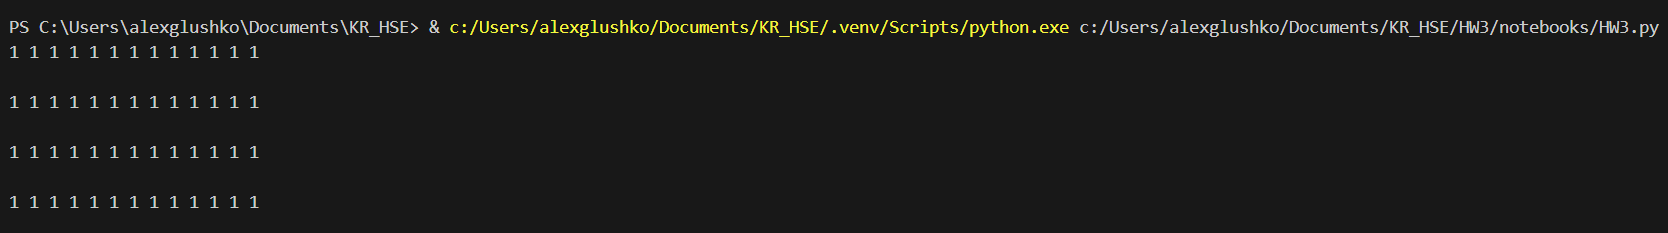
\includegraphics[width=\linewidth]{pictures/run_script.png}
    \caption{Результат работы кода}
    \label{fig:res}
\end{figure}















\end{document}